%%%%%%%%%%%%%%%%%%%%%%%%%%%%%%%%%%%%%%%%%%%%%%%%%%%%%%%%%%%%
%%  This Beamer template was created by Cameron Bracken.
%%  Anyone can freely use or modify it for any purpose
%%  without attribution.
%%
%%  Last Modified: January 9, 2009
%%

\documentclass[xcolor=x11names,compress]{beamer}
\usepackage[utf8]{inputenc}

%% General document %%%%%%%%%%%%%%%%%%%%%%%%%%%%%%%%%%
\usepackage{graphicx}
\usepackage{listings}
\usepackage{color}
\usepackage{mathtools}

\graphicspath{{diags/}}

\definecolor{gray}{rgb}{0.5,0.5,0.5}

\lstdefinelanguage{RLamb}{
    morekeywords={let,letregion,in,end,at,void,int},
    literate={->}{\ensuremath{\rightarrow}~}2
             {<=}{\ensuremath{\leq}~}2    {>=}{\ensuremath{\geq}~}2
             {R}{\ensuremath{\rho}}1
             {R1}{\ensuremath{\rho_1}}1   {R2}{\ensuremath{\rho_2}}1
             {R3}{\ensuremath{\rho_3}}1   {R4}{\ensuremath{\rho_4}}1
             {R5}{\ensuremath{\rho_5}}1   {R6}{\ensuremath{\rho_6}}1
             {RH}{\ensuremath{\rho_H}}1   {RL}{\ensuremath{\rho_L}}1
             {A}{\ensuremath{a~}}1        {N}{\ensuremath{n~}}1
             {P}{\ensuremath{p~}}1        {X}{\ensuremath{x~}}1
             {Y}{\ensuremath{y~}}1        {Z}{\ensuremath{z~}}1
             {\('L\)}{\ensuremath{_L}~}1
             {\\:}{\ensuremath{\lambda}}1,
    sensitive=f,
}[keywords,comments,strings]

\lstset{
    language=RLamb,
    aboveskip=3mm,
    belowskip=3mm,
    basicstyle={\small\ttfamily},
    breakatwhitespace=true,
    columns=flexible,
    escapeinside={(@}{@)},
    frame=l,
    keepspaces=true,
    numbers=left,
    numberstyle=\tiny\color{gray},
    showstringspaces=false,
    tabsize=4,
    xleftmargin=4pt
}

\definecolor{code}{RGB}{220, 20, 20}

\newcommand{\snippet}[1] {\textcolor{code}{\texttt{#1}}}
%%%%%%%%%%%%%%%%%%%%%%%%%%%%%%%%%%%%%%%%%%%%%%%%%%%%%%

%% Beamer Layout %%%%%%%%%%%%%%%%%%%%%%%%%%%%%%%%%%
\useoutertheme[subsection=false,shadow]{miniframes}
\useinnertheme{default}
\usefonttheme{serif}
\usepackage{palatino}

\setbeamerfont{title like}{shape=\scshape}
\setbeamerfont{frametitle}{shape=\scshape}

\setbeamercolor*{lower separation line head}{bg=DeepSkyBlue4} 
\setbeamercolor*{normal text}{fg=black,bg=white} 
\setbeamercolor*{alerted text}{fg=red} 
\setbeamercolor*{example text}{fg=black} 
\setbeamercolor*{structure}{fg=black} 
 
\setbeamercolor*{palette tertiary}{fg=black,bg=black!10} 
\setbeamercolor*{palette quaternary}{fg=black,bg=black!10} 

\renewcommand{\(}{\begin{columns}}
\renewcommand{\)}{\end{columns}}
\newcommand{\<}[1]{\begin{column}{#1}}
\renewcommand{\>}{\end{column}}
%%%%%%%%%%%%%%%%%%%%%%%%%%%%%%%%%%%%%%%%%%%%%%%%%%

\title{Static Methods for Memory Management}
%\subtitle{SUBTITLE}

\author{John~C~F}
 
\institute{
    
\includegraphics[width=5em]{iitb-black}
    \\
    Computer Science \& Engineering\\
    IIT Bombay
}

\date{
	\vspace{0.6cm}
	\today
}

\begin{document}

%%%%%%%%%%%%%%%%%%%%%%%%%%%%%%%%%%%%%%%%%%%%%%%%%%%%%%
%%%%%%%%%%%%%%%%%%%%%%%%%%%%%%%%%%%%%%%%%%%%%%%%%%%%%%
\begin{frame}

\titlepage

\end{frame}

%%%%%%%%%%%%%%%%%%%%%%%%%%%%%%%%%%%%%%%%%%%%%%%%%%%%%%
%%%%%%%%%%%%%%%%%%%%%%%%%%%%%%%%%%%%%%%%%%%%%%%%%%%%%%
\begin{frame}{Outline}
\tableofcontents
\end{frame}

%%%%%%%%%%%%%%%%%%%%%%%%%%%%%%%%%%%%%%%%%%%%%%%%%%%%%%
%%%%%%%%%%%%%%%%%%%%%%%%%%%%%%%%%%%%%%%%%%%%%%%%%%%%%%
\section{\scshape Introduction}
\begin{frame}{Introduction}
    \begin{itemize}
        \item Humans cannot be trusted with memory!
        \pause
        \item Garbage collection can get too slow!
        \pause
        \item Enter static analysis
        \begin{itemize}
            \item Regions
            \item Linear Types
        \end{itemize}
    \end{itemize}
\end{frame}

%%%%%%%%%%%%%%%%%%%%%%%%%%%%%%%%%%%%%%%%%%%%%%%%%%%%%%
%%%%%%%%%%%%%%%%%%%%%%%%%%%%%%%%%%%%%%%%%%%%%%%%%%%%%%
\section{\scshape RBMM}
\subsection{Definition}
\begin{frame}{Region-Based Memory Management}
    \begin{columns}[T]
        \begin{column}{.40\textwidth}
            \begin{figure}[h]
                \centering
                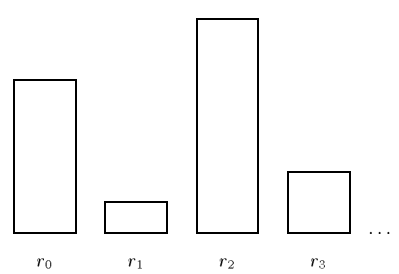
\includegraphics[width=0.96\textwidth]{regions-blocks.png}
                \caption{Stack of regions}
            \end{figure}
        \end{column}
        \hfill
        \begin{column}{.56\textwidth}
            \begin{itemize}
                \item Extended stack-based approach
                \begin{itemize}
                    \item Simpler runtime
                \end{itemize}
                \item Regions do not shrink
                \begin{itemize}
                    \item Pop whole
                \end{itemize}
                \item Associated with a lexical scope
                \pause
                \item Approaches
                \begin{itemize}
                    \item Translation-based
                    \item User-defined
                \end{itemize}
            \end{itemize}
        \end{column}
    \end{columns}
\end{frame}

%%%%%%%%%%%%%%%%%%%%%%%%%%%%%%%%%%%%%%%%%%%%%%%%%%%%%%
%%%%%%%%%%%%%%%%%%%%%%%%%%%%%%%%%%%%%%%%%%%%%%%%%%%%%%
\subsection{Example}

\begin{frame}[fragile]{Regions: Translation Example}
\begin{lstlisting}
let X = (2, 3) in (\:Y.(fst X, Y)) end 5
\end{lstlisting}
\pause
Gets translated to:

\begin{lstlisting}
letregion R4, R5
in  letregion R6
    in  let X = (2 at R2, 3 at R6) at R4
        in  (\:Y.(fst X, Y) at R1) at R5
        end
    end
    5 at R3
end
\end{lstlisting}
\end{frame}

\begin{frame}[fragile]{Regions: Translation Example}
\begin{lstlisting}
(@\snippet{let $x$ = (2, 3) in ($\lambda y$.(fst $x$, $y$)) end 5}@)
\end{lstlisting}

Gets translated to:

\begin{lstlisting}
letregion R4, R5
in  letregion R6
    in  (@\snippet{let $x$ = (2}@) at R2(@\snippet{, 3}@) at R6(@\snippet{)}@) at R4
        (@\snippet{in~~($\lambda y$.(fst $x$, $y$)}@) at R1(@\snippet{)}@) at R5
        (@\snippet{end}@)
    end
    (@\snippet{5}@) at R3
end
\end{lstlisting}
\end{frame}

%%%%%%%%%%%%%%%%%%%%%%%%%%%%%%%%%%%%%%%%%%%%%%%%%%%%%%
%%%%%%%%%%%%%%%%%%%%%%%%%%%%%%%%%%%%%%%%%%%%%%%%%%%%%%
\begin{frame}[fragile]{Regions: Translation Example}{Execution}
\begin{lstlisting}
letregion R4, R5
in  letregion R6
    in  let X = (2 at R2, 3 at R6) at R4
        in  (\:Y.(fst X, Y) at R1) at R5
        end
    end
    5 at R3
end
\end{lstlisting}

\begin{figure}[h]
    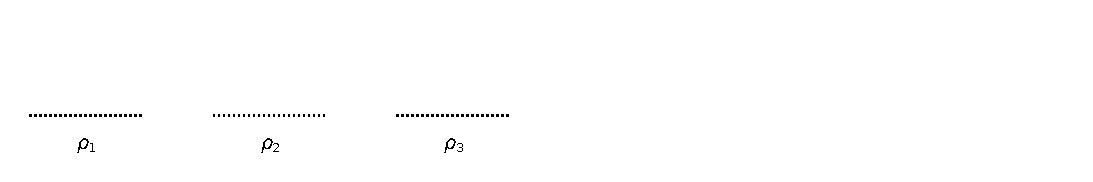
\includegraphics[width=\textwidth]{regions-1}
\end{figure}
\end{frame}

\begin{frame}[fragile]{Regions: Translation Example}{Execution}
\begin{lstlisting}
letregion R4, R5
in  (@\snippet{letregion $\rho_6$}@)
    in  let X = (2 at R2, 3 at R6) at R4
        in  (\:Y.(fst X, Y) at R1) at R5
        end
    end
    5 at R3
end
\end{lstlisting}

\begin{figure}[h]
    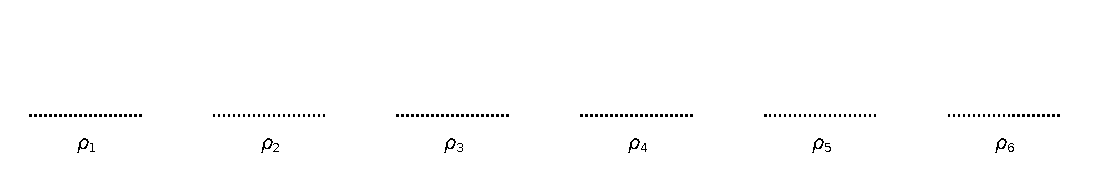
\includegraphics[width=\textwidth]{regions-2}
\end{figure}
\end{frame}

\begin{frame}[fragile]{Regions: Translation Example}{Execution}
\begin{lstlisting}
letregion R4, R5
in  letregion R6
    in  (@\snippet{let $x$ = (2 at $\rho_2$, 3 at $\rho_6$) at $\rho_4$}@)
        in  (\:Y.(fst X, Y) at R1) at R5
        end
    end
    5 at R3
end
\end{lstlisting}

\begin{figure}[h]
    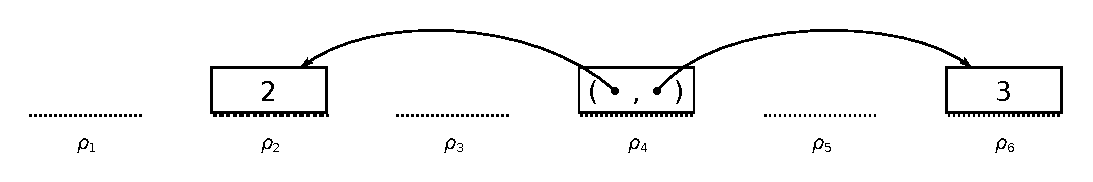
\includegraphics[width=\textwidth]{regions-3}
\end{figure}
\end{frame}

\begin{frame}[fragile]{Regions: Translation Example}{Execution}
\begin{lstlisting}
letregion R4, R5
in  letregion R6
    in  let X = (2 at R2, 3 at R6) at R4
        in  (@\snippet{($\lambda y$.(fst $x$, $y$) at $\rho_1$) at $\rho_5$}@)
        end
    end
    5 at R3
end
\end{lstlisting}

\begin{figure}[h]
    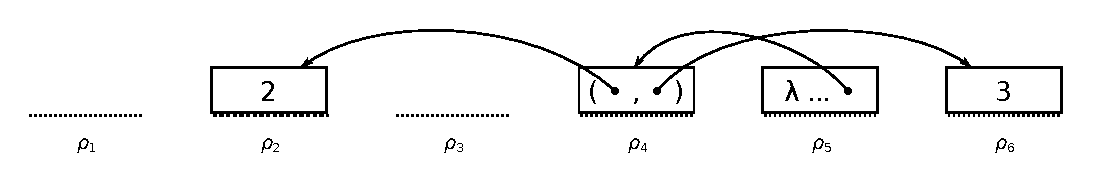
\includegraphics[width=\textwidth]{regions-4}
\end{figure}
\end{frame}

\begin{frame}[fragile]{Regions: Translation Example}{Execution}
\begin{lstlisting}
letregion R4, R5
in  letregion R6
    in  let X = (2 at R2, 3 at R6) at R4
        in  (\:Y.(fst X, Y) at R1) at R5
        end
    (@\snippet{end}@)
    5 at R3
end
\end{lstlisting}

\begin{figure}[h]
    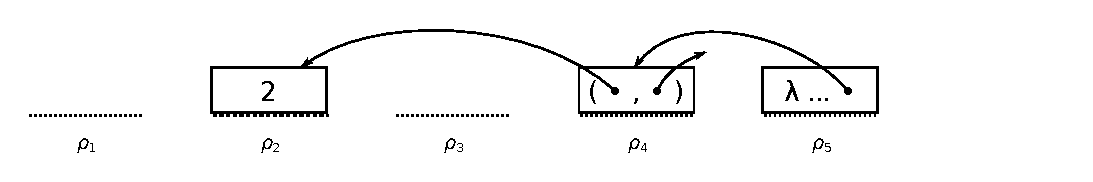
\includegraphics[width=\textwidth]{regions-5}
\end{figure}
\end{frame}

\begin{frame}[fragile]{Regions: Translation Example}{Execution}
\begin{lstlisting}
letregion R4, R5
in  letregion R6
    in  let X = (2 at R2, 3 at R6) at R4
        in  (\:Y.(fst X, Y) at R1) at R5
        end
    end
    (@\snippet{5 at $\rho_3$}@)
end
\end{lstlisting}

\begin{figure}[h]
    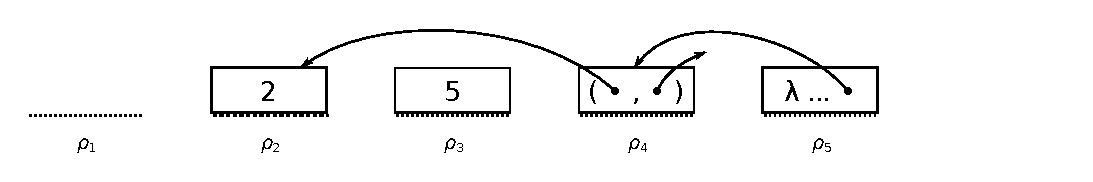
\includegraphics[width=\textwidth]{regions-6}
\end{figure}
\end{frame}

\begin{frame}[fragile]{Regions: Translation Example}{Execution}
\begin{lstlisting}
letregion R4, R5
in  letregion R6
    in  let X = (2 at R2, 3 at R6) at R4
        in  (@\snippet{($\lambda y$.(fst $x$, $y$) at $\rho_1$) at $\rho_5$}@)
        end
    end
    (@\snippet{5 at $\rho_3$}@)
end
\end{lstlisting}

\begin{figure}[h]
    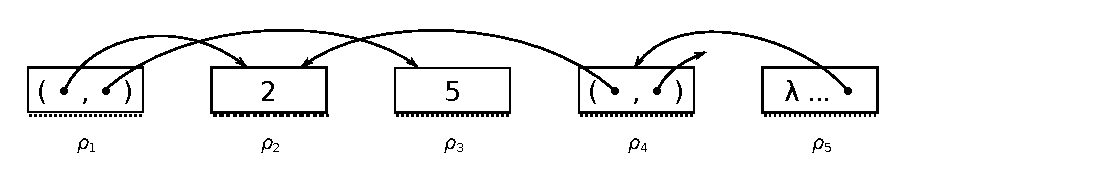
\includegraphics[width=\textwidth]{regions-7}
\end{figure}
\end{frame}

\begin{frame}[fragile]{Regions: Translation Example}{Execution}
\begin{lstlisting}
letregion R4, R5
in  letregion R6
    in  let X = (2 at R2, 3 at R6) at R4
        in  (\:Y.(fst X, Y) at R1) at R5
        end
    end
    5 at R3
(@\snippet{end}@)
\end{lstlisting}

\begin{figure}[h]
    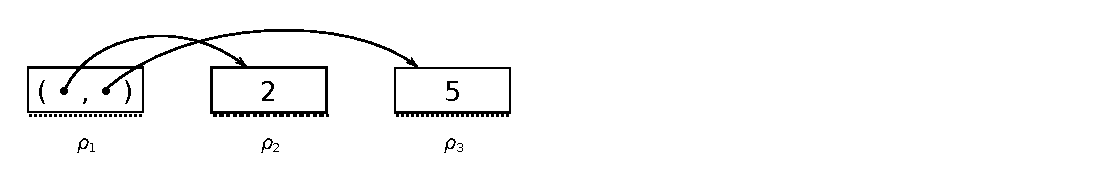
\includegraphics[width=\textwidth]{regions-8}
\end{figure}
\end{frame}

%%%%%%%%%%%%%%%%%%%%%%%%%%%%%%%%%%%%%%%%%%%%%%%%%%%%%%
%%%%%%%%%%%%%%%%%%%%%%%%%%%%%%%%%%%%%%%%%%%%%%%%%%%%%%
\section{\scshape Region Inference}
\subsection{Key Ideas}
\begin{frame}{Region Inference}{Key Ideas}
    \begin{itemize}
        \item Closures can capture local environments
        \pause
        \item Thus region accesses must be analyzed
        \pause
        \item Introduce an ``Effect System" to represent region accesses
        % TODO small example
        \pause
        \item ``Effects" should be part of the type of closures
        % TODO small example
        \pause
        \item If the type (+place) of an expr does not contain $\rho$, then
        \pause
        \begin{itemize}
            \item Either $\rho$ is not accessed within
            \pause
            \item Or $\rho$ does not escape outside
        \end{itemize}
    \end{itemize}
\end{frame}

%%%%%%%%%%%%%%%%%%%%%%%%%%%%%%%%%%%%%%%%%%%%%%%%%%%%%%
%%%%%%%%%%%%%%%%%%%%%%%%%%%%%%%%%%%%%%%%%%%%%%%%%%%%%%
\subsection{Limitations}
\begin{frame}{Limitations}
    \begin{itemize}
        \item Whole program inference is bad!
    \end{itemize}
\end{frame}

%%%%%%%%%%%%%%%%%%%%%%%%%%%%%%%%%%%%%%%%%%%%%%%%%%%%%%
%%%%%%%%%%%%%%%%%%%%%%%%%%%%%%%%%%%%%%%%%%%%%%%%%%%%%%
\section{\scshape Cyclone}
\subsection{User-defined regions}
\begin{frame}{Cyclone}{User-defined regions}
    {\large Goals}
    \begin{itemize}
        \item Fine-grained control over resources
        \item Minimal inference -- no hidden meanings!
        \item Provably-safe C-dialect
    \end{itemize}
\end{frame}

%%%%%%%%%%%%%%%%%%%%%%%%%%%%%%%%%%%%%%%%%%%%%%%%%%%%%%
%%%%%%%%%%%%%%%%%%%%%%%%%%%%%%%%%%%%%%%%%%%%%%%%%%%%%%
\subsection{Limitations}
\begin{frame}{Cyclone: Limitations}
    Multi-threading and list of chunks
\end{frame}

%%%%%%%%%%%%%%%%%%%%%%%%%%%%%%%%%%%%%%%%%%%%%%%%%%%%%%
%%%%%%%%%%%%%%%%%%%%%%%%%%%%%%%%%%%%%%%%%%%%%%%%%%%%%%
\section{\scshape Linear Types}
\subsection{Definition}
\begin{frame}{Linear Types: Definition}
    \begin{itemize}
        \item Each object must be consumed exactly once
    \end{itemize}
\end{frame}

%%%%%%%%%%%%%%%%%%%%%%%%%%%%%%%%%%%%%%%%%%%%%%%%%%%%%%
%%%%%%%%%%%%%%%%%%%%%%%%%%%%%%%%%%%%%%%%%%%%%%%%%%%%%%
\subsection{Relaxing Constraints}
\begin{frame}{Linear Types: Relaxing Constraints}
    
\end{frame}

%%%%%%%%%%%%%%%%%%%%%%%%%%%%%%%%%%%%%%%%%%%%%%%%%%%%%%
%%%%%%%%%%%%%%%%%%%%%%%%%%%%%%%%%%%%%%%%%%%%%%%%%%%%%%
\subsection{Borrowing}
\begin{frame}{Borrowing}
    
\end{frame}

\end{document}